\begin{homeworkProblem}
  Representar gráficamente:
  $$(1-2i)+(-3+i);(2+i)(-1+2i);\frac{-2+4i}{1-3i}$$
  \begin{solution}
    Note que:
    \begin{enumerate}
      \item $(1-2i)+(-3+i)=(1-3)+(-2+1)i=-2-i$.
      \item $(2+i)(-1+2i)=[(2)(-1)-(1)(2)]+[(2)(2)+(-1)(1)]i=-4+3i$.
      \item $\frac{-3+4i}{1-3i}=\frac{(-2+4i)(1+3i)}{1+9}=\frac{-14-2i}{10}=-\frac{7}{5}-\frac{1}{5}i$
    \end{enumerate}
    que gráficamente se ven de la siguiente forma en su expresión en el plano complejo:
    \begin{center}
      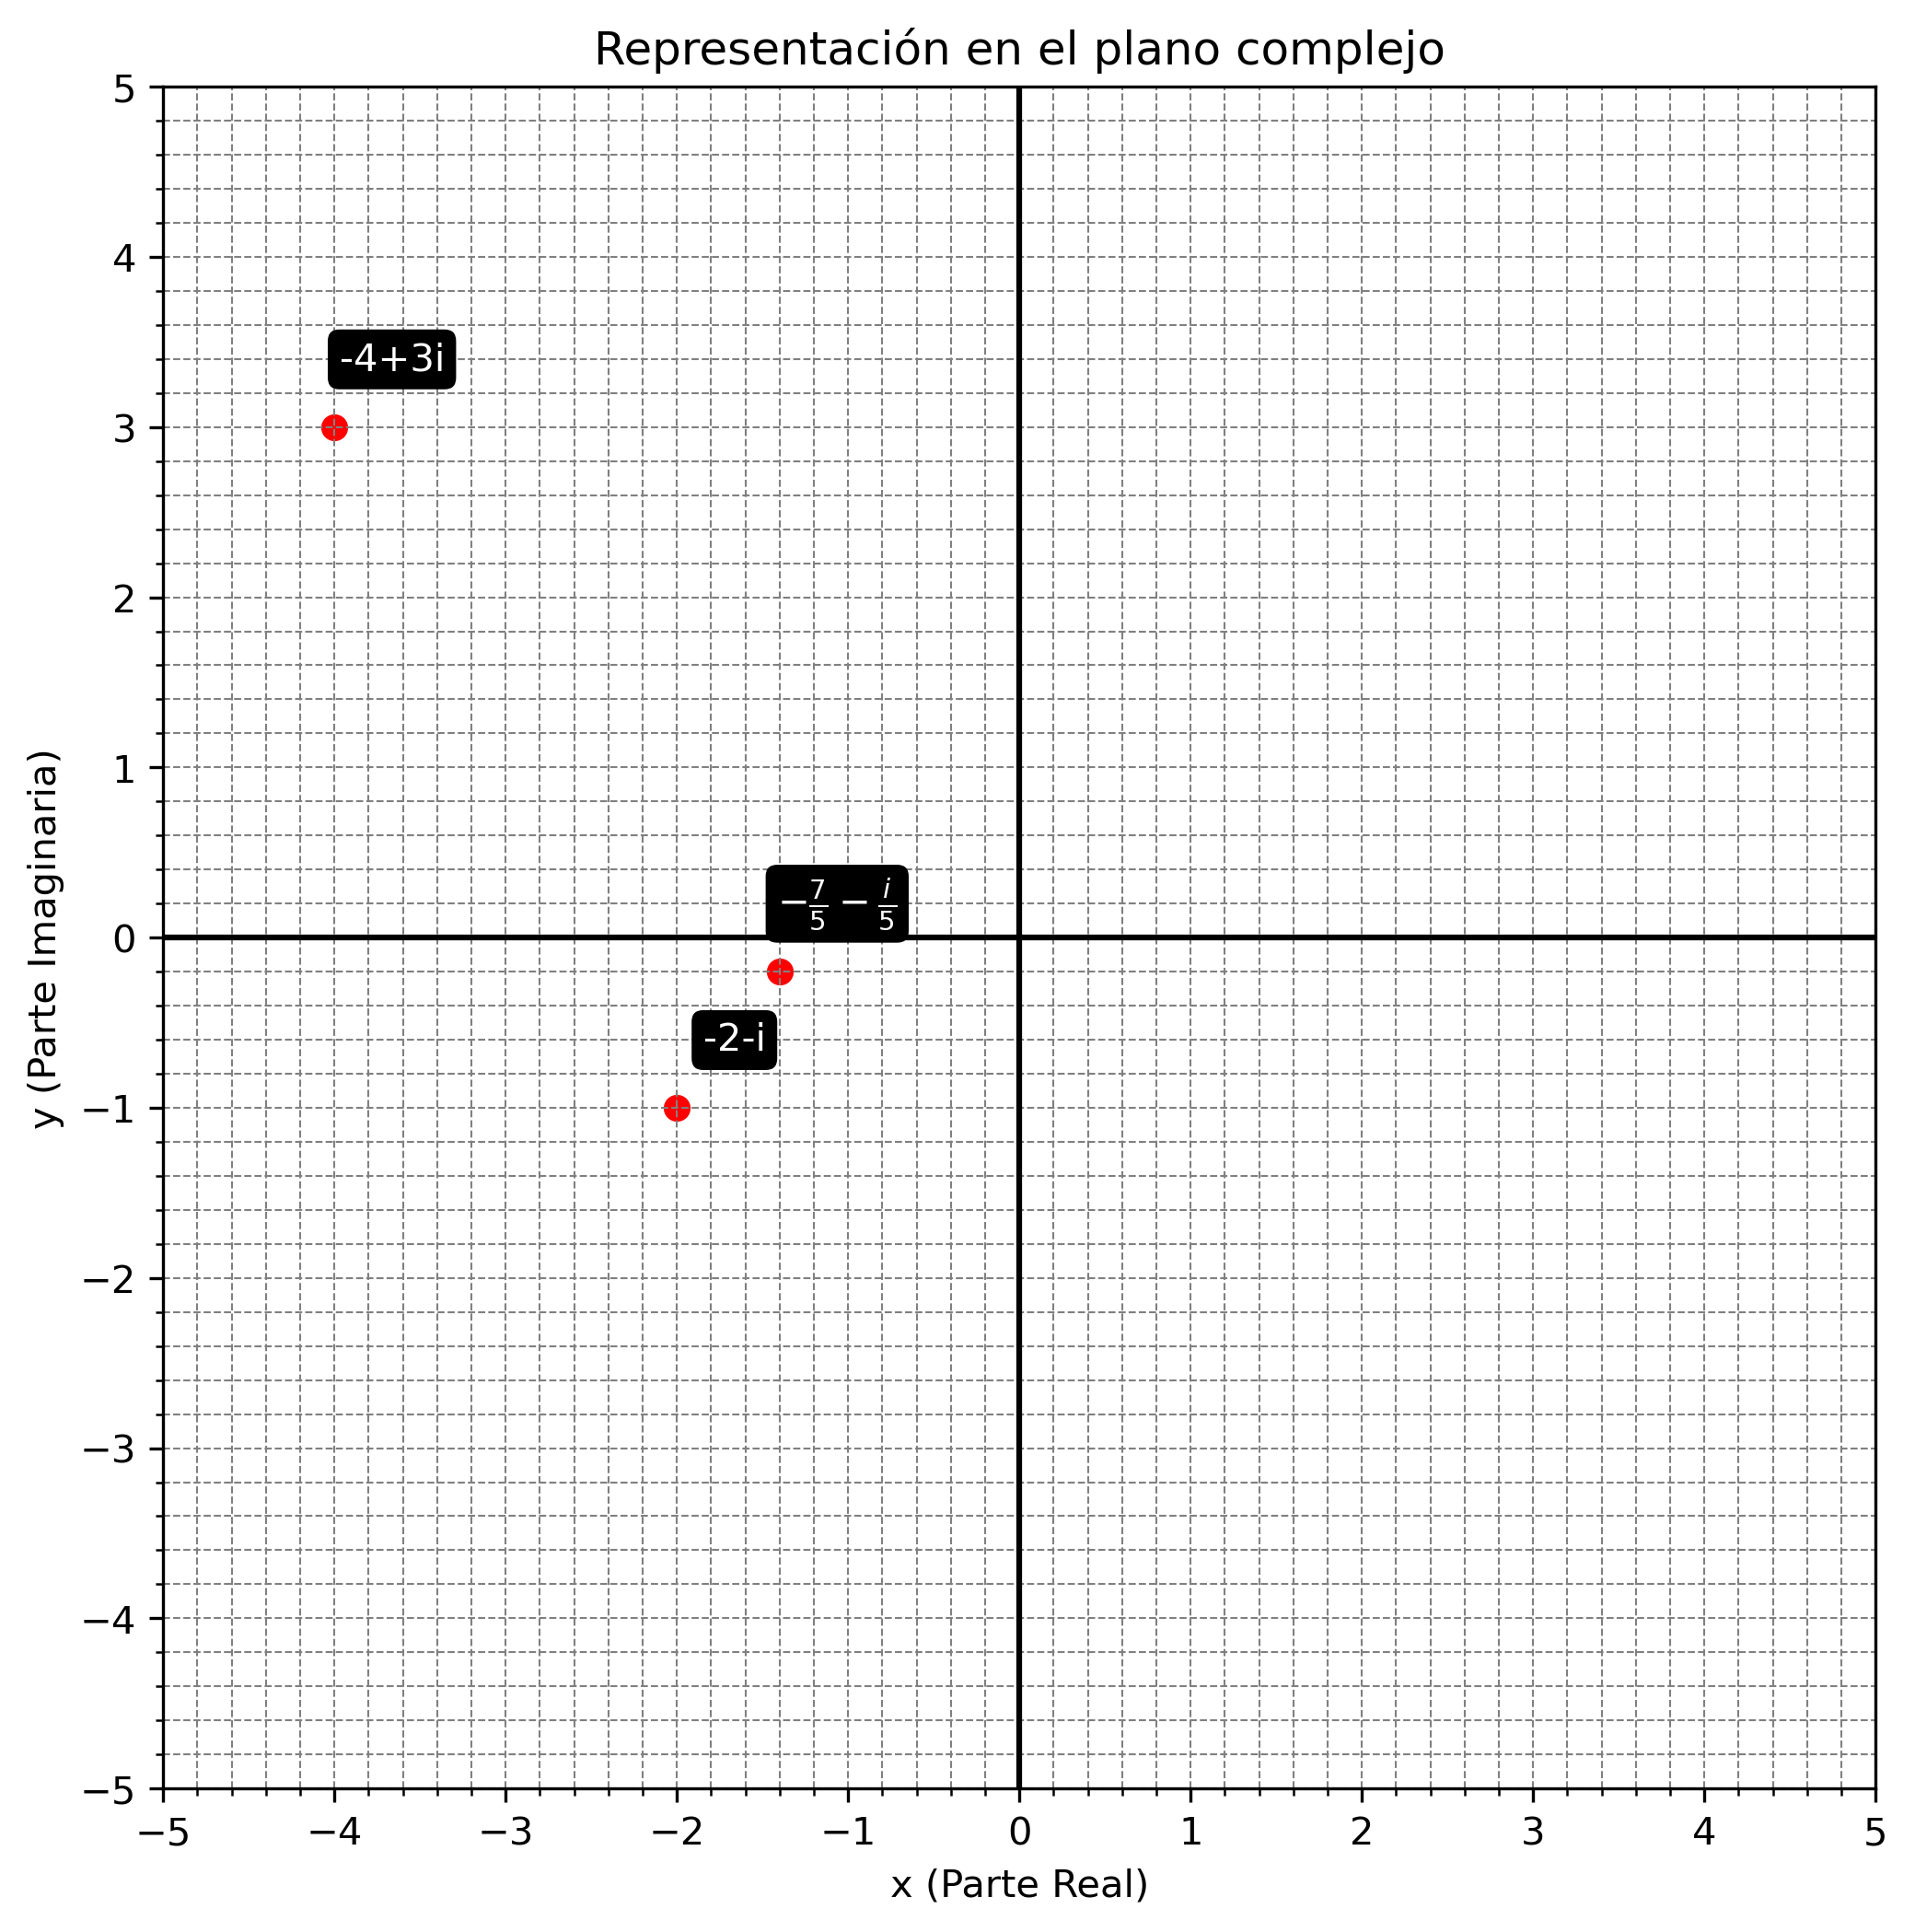
\includegraphics[scale=0.5]{images/grafico_punto_1.png}    
    \end{center}
  \end{solution}
\end{homeworkProblem}
